\documentclass[11pt]{article}
\usepackage{graphicx}
\usepackage[T1]{fontenc}
\usepackage{txfonts}
\setcounter{secnumdepth}{0}
\usepackage[affil-it]{authblk}   % author affiliation
\usepackage{lineno} %line numbers
\usepackage[a4paper, total={6.5in, 8.5in}]{geometry} % set page size
\usepackage{setspace}
\doublespacing


\begin{document}

\title{Demographic Bias in Human Cell Studies }
\author{Jessica Snyder\textsuperscript{1}, Iva Bojic\textsuperscript{1,2}, Aarom Gerow\textsuperscript{3}, Carlo Ratti  \textsuperscript{1,2 } \\ \textsuperscript{1}Massachusetts Institute of Technology, SENSEable City Lab \\ \textsuperscript{2}Singapore-MIT Alliance for Research and Technology \\  \textsuperscript{3}The University of Chicago, Knowledge Lab }

\maketitle

\linenumbers
\begin{abstract} \end{abstract}


\section{Rationale}
The long term consequences of medical research is those demographics most heavily represented as donors to biopsies used in lab work have the best prognosis for treatment. Targeted breast cancer therapies and preventative screening sensitive to various tumor are required to absolve demographic inequalities in breast cancer treatment \cite{batina2013variation}.  When breast cancer patients are grouped by ethnicity, black patients are less likely to survive than other ethnicities. Leading research hypothesizes some part of black patient's decreased breast cancer survival rate is due to due to diagnosis at a later stage, as well as the cancer growing at a faster rate and were more likely to spread \cite{batina2013variation}. Intrinsic factors, biological properties of the disease itself, and not just extrinsic factors, access to care, effect the efficacy of breast cancer treatment. The importance of intrinsic factors justifies a proportional and parallel research effort using cell lines from black patients for effective treatment.

\cite{brennan2012there}

Generating credible cell-based data has historically relied on consensus-building  using a catalog of synonymous cell lines \cite{yu2015resource}. 
 
 Biomedical vocabularies

Environmental exposure and genetic background determine the breast cancer's subtypes, aggressiveness and prognosis. 
Alternative treatment options for patients with a genetic predisposition for hormone receptor-negative breast cancers, which are also likely black, is  limited \cite{huo2009population}. Highly agressive tumor subtypes are coorelated to risk factors such as obesity, which disproportionately effects black women. 

Access to high quality hospital care is known to effect breast cancer survival rate, coupling economic status with prognosis, adversely effecting black patients \cite{shavers2003racial}.  Self-reported race coorellated to breast cancer properties, such as estrogen receptor status and stage of diagnosis, more than percent African ancestry, suggesting social determinants shape the disease physiology more than genetic predispositions \cite{reding2012examination}.

A data-driven retrospective on disease burden and treatment effectiveness to guide medical research funding and health policy decisions towards the most productive population-level outcomes \cite{kim2016cancer}. 
 Racial difference in the efficacy of breast cancer treatment cause black woman to have a higher risk of dying than other ethnicites, the higher risk for death is consistent in all-cause and cardiovascular disease death \cite{berkman2014racial}.
 
Methylation along the DNA strand stabilizes gene expression, without methylation irregular gene expression increases the risk of cancer  \cite{zhang2011significant}. Demographic and environmental factors dictate the gradation of methylation in peripheral blood cells, and therefore cancer risk and tumor properties. 


\begin{enumerate}
\item CDC statistic on on incidence and morbidity rates expose a disparity in the efficacy of treatment among demographic groups. 
\item Center for Disease Control (CDC) statistics show, since 1999, Caucasian patients are more likely to survive a breast cancer diagnosis than Black patients. 
\item The demographic most cited in human cell studies of breast cancer is the demographic with the highest survival rate. 
\item The same positive correlation, between the demographic-specificity of the source tissue and the efficacy of the eventual medical treatment, is observed in prostate cancer
\end{enumerate}

\section{Building the database}
Cell lines are well-recognized models to study disease, especially cancer. 

Cross-contamination of a cell line by another cell line cancels its utility as a standard, representative of the original donor, tissue and cell type. Therefore, accepted practice requires such cell lines be omitted from research. \cite{capes2010check}. In this retrospective, we disregard contaminated cell lines, regardless of when the contamination occurred. Of the 336 most popular cell lines surveyed, 23 were disregarded, due to inclusion on International Cell Line Authentication Committee's Database of Cross-contaminated or Misidentified Cell Lines. 


\begin{figure}[h!]
\centering
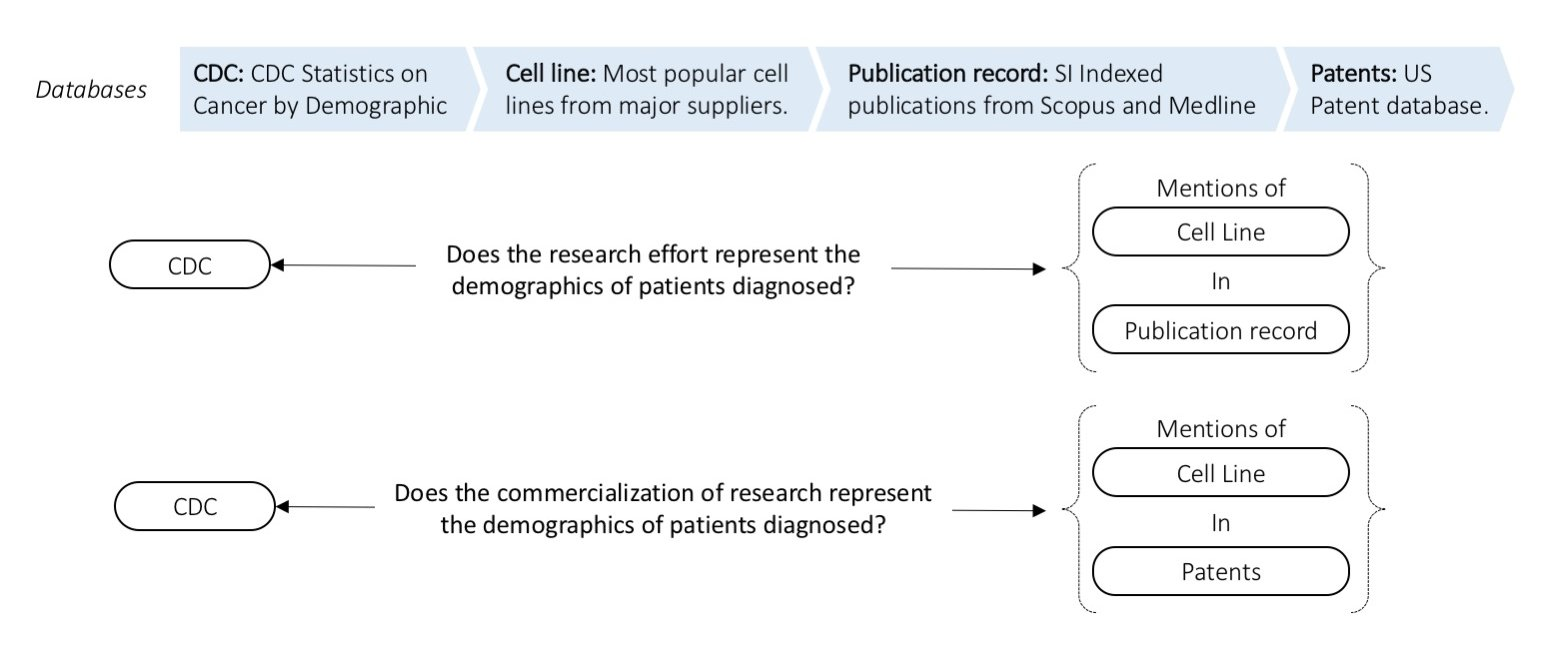
\includegraphics[width=0.98\columnwidth]{Databases.jpg}
\caption{\label{dist2} Diagram of databases to compare the cancer patient population to research efforts and commercialization. }
\end{figure}


\section{The available human cell lines}

 The first human cells to maintain phenotypic stability after a year in vitro were from a cervical cancer biopsy, achieving the first human "cancer in a test tube", used since as a standard for medical research \cite{gey1952tissue}.

\begin{enumerate}
\item A timeline of when cell lines were introduced, and the demographics of the donor.
\item Conclusion: Beginning in the 1950s, cell line were established from black females, followed by Caucasian men and women in the 60?s, Asian in 80?s, and Hispanic in the 90?s. 

\end{enumerate}
A significant majority of publications use cell lines \cite{arlett2001use}.
\section{Demographic inclusiveness of the publication record}


"Human cancer in a test tube" provide a standard for genotypic and phenotypic stability. Cross-contamination of cell lines causes falsified data, this is a failing of the peer review process to require authentication of the cell line as part of the experimental method  \cite{masters2002hela}. 

\cite{eid2012current}

\begin{enumerate}
\item A timeline of the number of publications in the Medline and/or Scopus database, indexed with the MESH term ''Breast Neoplasms'' shows \textgreater 120k publications citing human cell lines derived from breast cancer since the late 70's. The demographic representation in the publication record shows \textgreater 95\% of publications cite a Caucasian cell line, despite the availability of alternatives. 

\item The same trend, a majority of publications citing a human cell line were sourced from Caucasian donors, is true for prostate and lung cancer. 
Calculate the demographic bias in the publication records. Subtract the proportion of people diagnosed with cancer for each demographic from the proportion of papers citing a human cell line derived from a donor of the same demographic. 
\end{enumerate}

\section{Defining bias.}

\begin{equation} \label{simple_equation}
    \alpha = \sqrt{ \beta }
\end{equation}

\begin{enumerate}
\item  According to the afore defined demographic bias, Caucasian are over-represented compared to other races. The bias in favor of Caucasian in breast cancer research using human cell lines has risen from 15-20\% since 1999.  
\item A similar bias exists in prostate cancer research, the bias in favor of Caucasian has risen from 10-15\% since 1999.
\end{enumerate}

\section{Commercialization of the research effort}
US Patents cite fewer unique cell lines than the publication database, meaning patents rely on a more uniform set of cell line models than publications, homogenizing the research standards used to substantiate claims, increasing the gap between population-level genetic diversity and medical research based on cell models. 

Figure \ref{CDF} presents the cumulative distribution function 

\begin{figure}[h!]
\centering
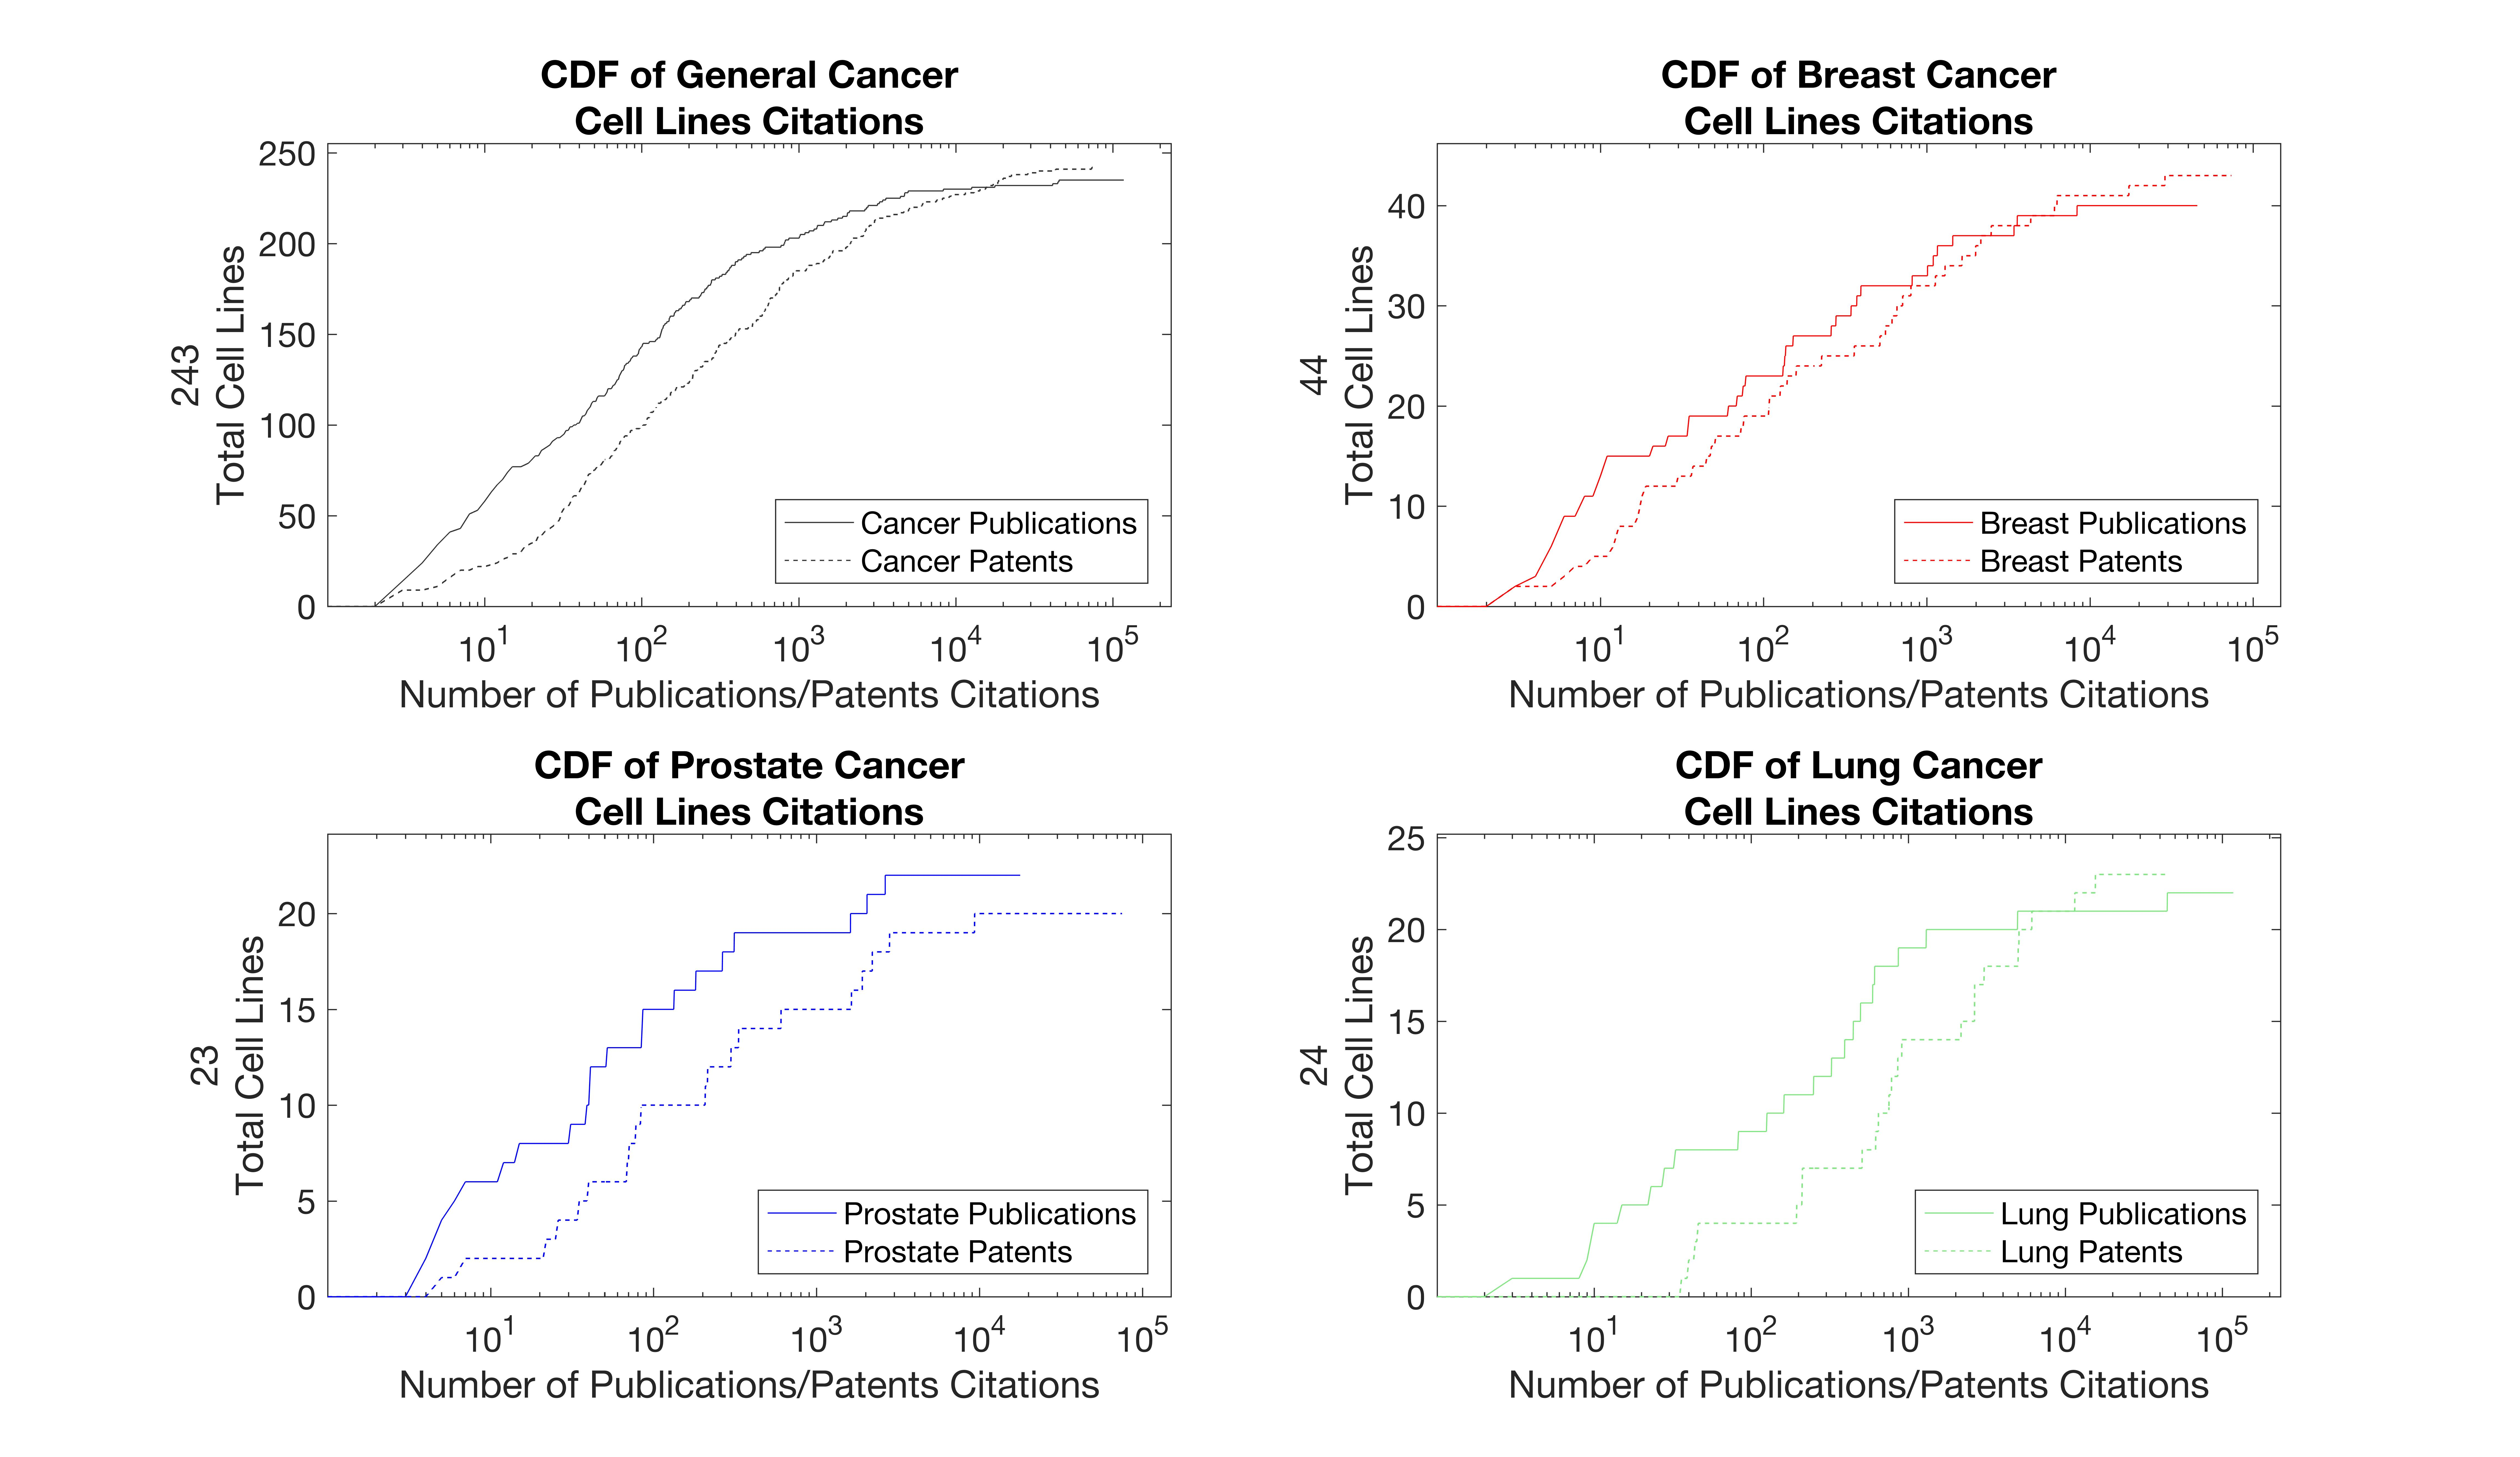
\includegraphics[width=1\columnwidth, trim={20cm 20 60 20}, clip]{CDF.jpg}
\caption{\label{CDF} Cumulative distribution function (CDF) of the number of publications and patents citing human cell lines for all cancer types, breast, prostate and lung. }
\end{figure}




\section{Forging ahead}

Summary and call to action
Transformative approaches to health care, such as personalized medicine, authenticate the importance of genetic variation on the effectiveness of treatment, physicians use genomic analysis to determine the course of treatment, circumventing the limitations of generalized treatments with tailored treatments. Here, we survey the genetic variation in breast cancer research with human cell models by characterizing the demographics of cell line donors represented in breast cancer research. 




\bibliographystyle{unsrt}
\bibliography{refs}

\end{document}